\chapter{Communicators}

In the unmodified program, the process on the row being at the rank 0, that is in the column 0 since column number are used for ordering, transfers the row number to the other process in the same row. So, all the processes on a row will have their row number as data, as can be seen in the followig picture:
\begin{figure}[!h]
\begin{center}
	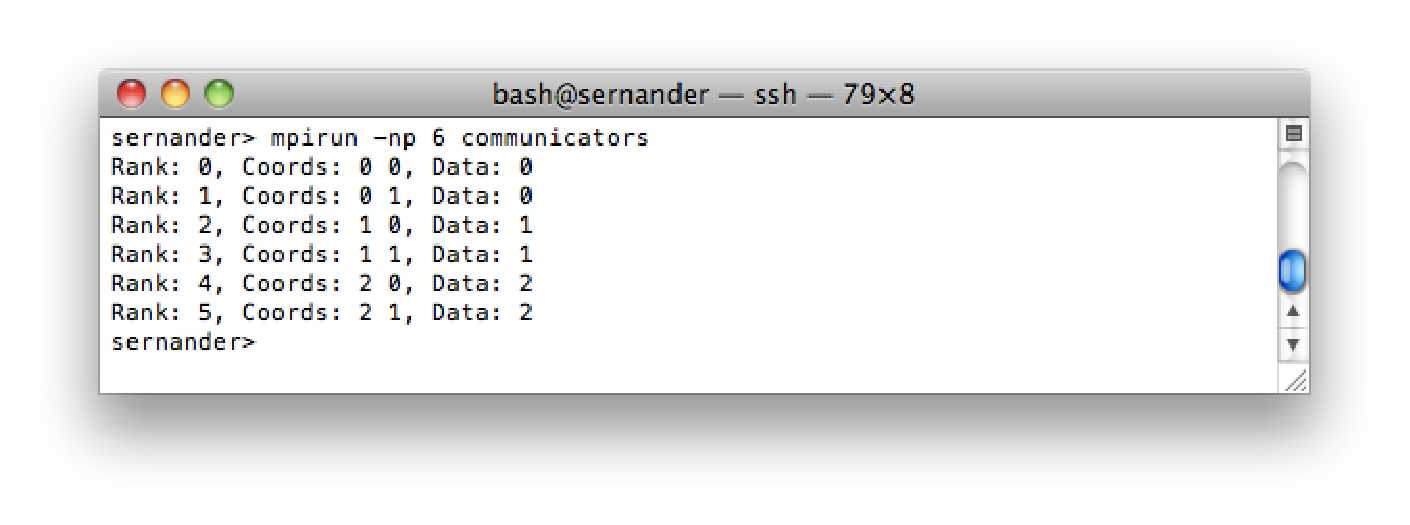
\includegraphics[width=\textwidth]{pic/row.eps}
	\caption{Communicator for each row}
\end{center}
\end{figure}

In the modified program, the communicator is declared in such a way that processes are grouped by column number and sorted by row number (the exact opposite as before). So, now, the first process of a column, the one being on the row 0, sends its row number to the processes in the same column. So, the value of every process becomes the row number of the rank 0 process in this column, that is 0. This is illustrated by the following screenshot:
\begin{figure}[!h]
\begin{center}
	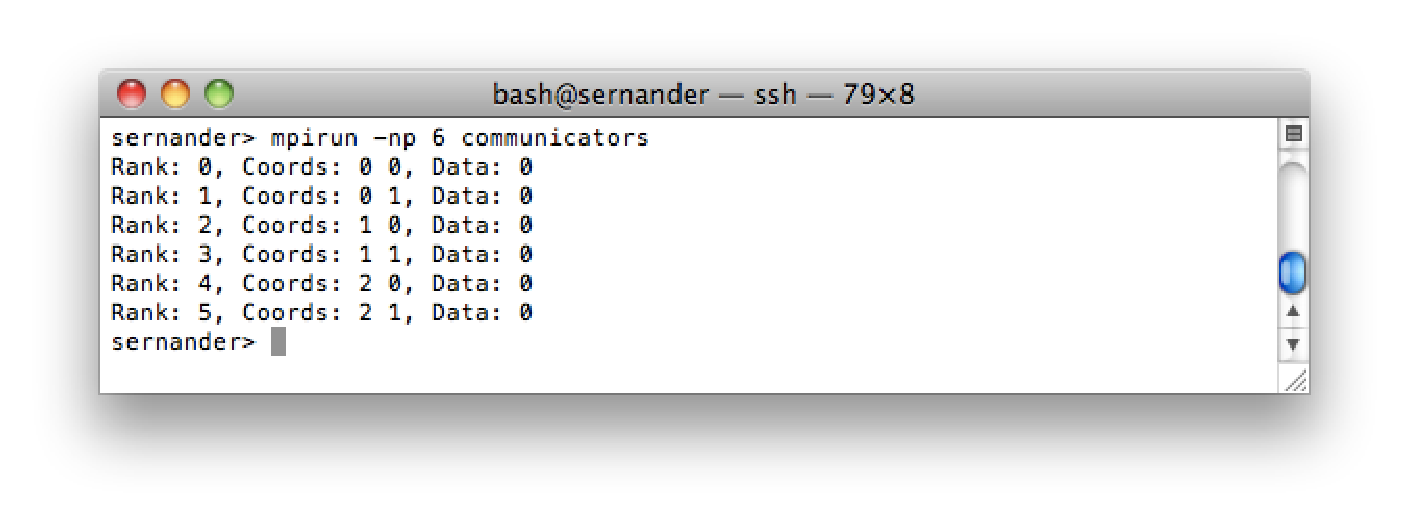
\includegraphics[width=\textwidth]{pic/col.eps}
	\caption{Communicator for each column}
\end{center}
\end{figure}

